\documentclass{article}
\title{\textbf{Machine Learning Notes}}
\author{}
\date{} 
\UseRawInputEncoding

\usepackage{graphicx}
% Links
\usepackage{hyperref}
\hypersetup{
    colorlinks=true,
    linkcolor=blue,
    filecolor=magenta,      
    urlcolor=cyan,
}
 
\urlstyle{same}

% Code Coloring
\usepackage{xcolor}
\usepackage{listings}
\lstset{
  language=bash,
  basicstyle=\small\sffamily,
  showstringspaces=false
  %numbers=left,
  %numberstyle=\tiny,
  numbersep=3pt,
  %linewidth=13cm,
  frame=tb,
  columns=fullflexible,
  backgroundcolor=\color{yellow!20},
  linewidth=1.4\linewidth,
  xleftmargin=0\linewidth
}


%Box Note
\usepackage{graphicx}
\usepackage{tcolorbox}
\tcbuselibrary{skins}
\usepackage{lipsum}
\definecolor{boxTitle}{HTML}{fff79a}
\definecolor{boxBackground}{HTML}{fffce0}
\definecolor{boxFrame}{HTML}{f1e2b8}

\tcbset{my box/.style={
    enhanced, fonttitle=\bfseries,
    colback=boxBackground, colframe=boxFrame,
    coltitle=black, colbacktitle=boxTitle,
    attach boxed title to top left={xshift=0.3cm,
                                    yshift*=-\tcboxedtitleheight/2},
    boxed title style={
      before upper=\hspace*{0.5cm}, % reserve space for the image
      overlay={
       \node at ([xshift=0.5cm]frame.west)
         {\includegraphics[scale=0.65]{bc-dodecaedre}};
      }
    }
  }
}

\newtcolorbox{mybox}[1][]{my box, #1}

\begin{document}
\maketitle
\tableofcontents{}
\section{Machine Learning Applications in real life}
\begin{itemize}
  \item Face Recognition in Facebook
  \item 
\end{itemize}

\subsection{Prerequisites and used libraries}

\subsection{Concept}
Features (independent variables) and dependent variables, the features which you are going to predict the dependent variables.\\
Median and Medium, Mean average:\\
Most Frequent Value\\
Best fit line\\
Regression V.s. Classification:
In regression we predict a value, but in classification we predict a category or class.\\
The ground truth is what you measured for your target variable for the training and testing examples (simply the observed independent variables in the test set and the training set).\\

\section{Data prepressing}
While working with the machine learning at any phase, this step is mandatory you have some data and you need to prepare it to work in a perfect phase.\\

\lstinputlisting[caption=example embed source]{resources/src/01-DataPrepressing/preprocessing.py}

\begin{enumerate}
  \item Deal with missing data using sklearn
  \item Deal with categorical data
  Using Label Encoder V.s. One-Hot Encoder:\\
  LabelEncoder can turn [dog,cat,dog,mouse,cat] into [1,2,1,3,2], but then the imposed ordinality means that the average of dog and mouse is cat. Still there are algorithms like decision trees and random forests that can work with categorical variables just fine and LabelEncoder can be used to store values using less disk space.\\

  One-Hot-Encoding has the advantage that the result is binary rather than ordinal and that everything sits in an orthogonal vector space. The disadvantage is that for high cardinality, the feature space can really blow up quickly and you start fighting with the curse of dimensionality. In these cases, I typically employ one-hot-encoding followed by PCA for dimensionality reduction. I find that the judicious combination of one-hot plus PCA can seldom be beat by other encoding schemes. PCA finds the linear overlap, so will naturally tend to group similar features into the same feature.\\

  \item Feature Scaling
  Why feature scaling, if there are different ranges in features then the features biased in the correlation computation might happen which means that features with high values might dominate the features with low values as the features with higher ranges might be having big impact on the dependent variables.\\
  
  In linear regression there is no need to apply a feature scaling as the features has coefficients and features with very high values will be compensated by low coefficients.

  Two techniques for feature scaling:

  \begin{center}
    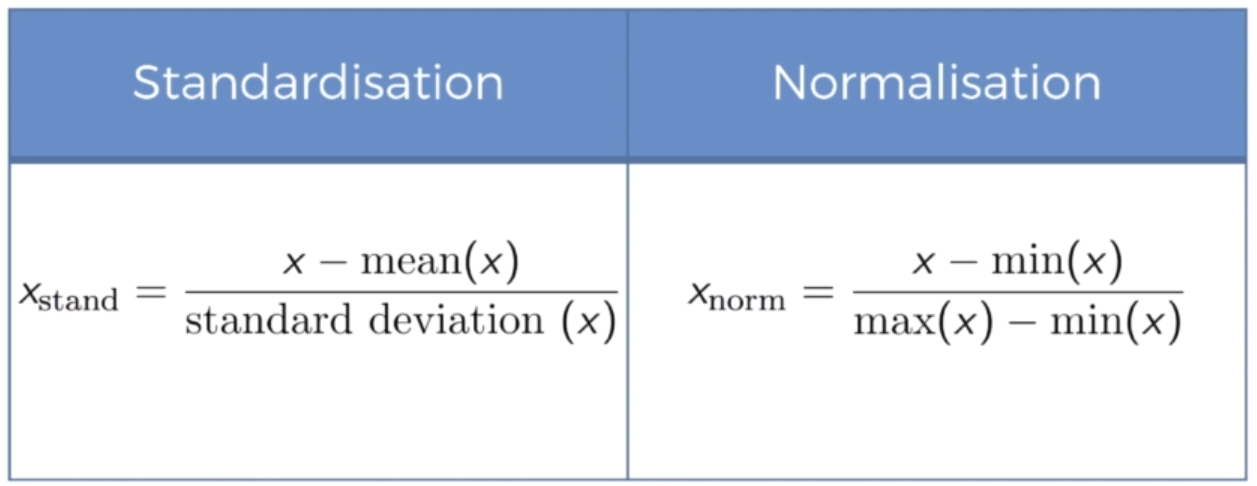
\includegraphics[scale=0.60]{./resources/img/01-preprossesing/featureScaling.PNG}
  \end{center}

  \begin{enumerate}
    \item Standardization
    As we divide on the standard deviation, the values will be between -x, +x
    \item Normalization
    it will put all the values between 0-1
  \end{enumerate}

  \item Split the dataset into training set and test set
  Splitting into two sets, 80\% used to train the model and 20\% to test it.\\
  We need to have the test set to overcome the overfitting with the training set, as the model trained too much on the training set and hence produces bad observations (it's like a student trained on a a lot of exams and certain models, but when a new exams with new models came out he fails)

\end{enumerate}

\section{Regression models}
regression analysis is a set of statistical processes for estimating the relationships between a dependent variable (often called the 'outcome variable') and one or more independent variables (often called 'predictors', 'covariates', or 'features').\\

This is the branch is used to predict a continuous numerical values (e.g. temperature, salary, ...)

Assumptions of linear regression: so before building a linear regression models, we need to check that these assumptions are true. 
\begin{enumerate}
  \item Linearity
  \item Homoscedasticity
  \item Multivariate normality
  \item Independence of errors
  \item Lack of multicollinearity
\end{enumerate}

\begin{itemize}
  \item Linear regression\\
    
  \subsection{Simple Linear regression} is simply the straight line equation \(y=b_0+b_1*x_1\) where y is the dependent variable, and x is the independent one and b is the coefficient.\\
    In linear regression we have one independent variable \(x\)
  
    Example: the relation between the salary and the years of experience.\\

    The best fitting line: it's the line with the smallest \textbf{sum(y-y\^)\^2} %\(\sum(y-y_^)^2\)

    \lstinputlisting[caption=example embed source]{resources/src/02-Regression-Models/01-LinearRegression/LinearRegression.py}

\subsubsection{Assumptions of linear regression models}
\begin{itemize}
  \item Linearity
  \item Homoscedasticity
  \item Multivariate normality
  \item Independence of errors
  \item Lack of multicollinearity
\end{itemize}

  \subsubsection{Multiple Linear regression models}
  It's a linear relationships between the dependent variables with more than one feature \(y=b_0+b_1*x_1+b_2*x_2 + ... + b_n*x_n\).

  Dummy Variables: 
  when we have a categorical variables as features, then it's hard to represent them in the linear regression equation, instead we create dummy variables with a chosen coefficient and a switch to switch between the states.\\
  
  Example:
  \begin{center}
    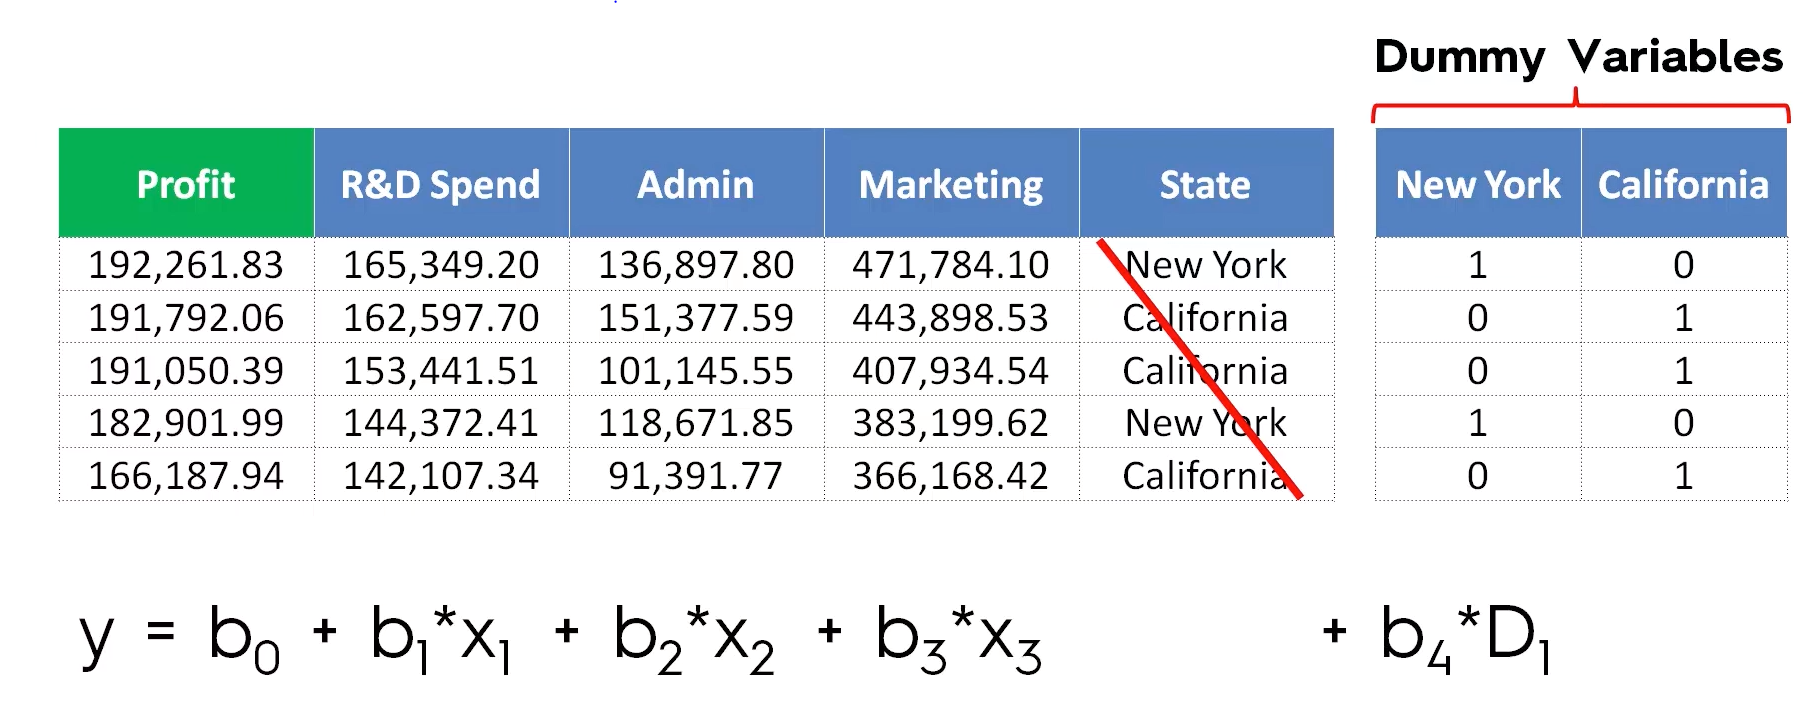
\includegraphics[scale=0.50]{./resources/img/02-regression/02-dummy-varaibles.PNG}
  \end{center}
  
  Dummy Variables trap:\\
  Always omit one dummy variable out of the equation, so if we have 100 variables, just include 100-1.

  Backward Elimination:\\
  Before to go further we need to know how to calculate the p-value.\\
  What is the null-hypothesis \(H_0\)?
  the p-value is used to reject the null-hypothesis, as if the p-value is too low so the null-hypothesis will be wrong which called a significant result (the alternative hypothesis), and if p value is large then the null-hypothesis is correct and this is non-significant result.

  Building a Model:\\
    In order to construct a reliable model, then we need first to decide which independent variables are important or which are not, which means that we might have some independent variables which are statistically significant, and others are not which might affect our model accuracy, we need need to keep only the ones with high statistically significant in our prediction, and the following methods are used to do so:
    \begin{enumerate}
      \item All-in
      You use this method if:  
      1. If you have a \textbf{prior knowledge} that you need to use them.\\
      2. If you have to use them all.\\
      3. Preparing to Backward Elimination.\\

      \item Backward Elimination
        1. Select a significance level to stay in the model (default SL = 0.05)\\
        2. Fit the full model with all possible predictors\\
        3. Consider the predictor with the highest P-value. if P > SL then go to no.4, otherwise go to FIN.\\
        4. Remove the predictor (remove the variable with the highest P-value)\\
        5. Fit model, without the removed variable.\\
        6. Repeat from 3 to 5 until the P-value > SL is not correct go to FIN so this step your model is prepared.\\

        By this we eliminate the number of variables till we 

      \item Forward Selection
        The opposite of backward one.
        1. Select a significance level to enter the model (e.g. SL = 0.05)\\
        2. Fit all \textbf{simple regression} models \(y ~ x_n\) Select the one with the lowest P-value.\\
        3. keep this variable and FIT all possible models with extra predictor added to the one(s) you already have.\\
        4. Consider the predicator with the lowest P-value the lowest P-value, if P < SL, go to STEP3, otherwise go to FIN.\\

      \item Bidirectional Elimination
        1. Select a significance level to enter and stay in the model e.g. SLENTER = 0.05, SLSTAY = 0.05\\
        2. Perform the next step of the forward Selection (new variables must have: P < SLENTER to enter).\\
        3. Perform ALL steps of backward elimination (old variables must have P < SLSTAY to stay).\\
        4. Move back to step 2, until you can't add new variables, and no variables can't be eliminated.\\

      \item Score Comparison
    \end{enumerate}

Note: step-wise regression refers to methods 2, 3, and 4.


\subsubsection{Polynomial Linear Regression}    
It's a special case of multiple linear regression, in this case we will be having the equation on the shape: \textbf{\(y=b_0,b_1*x_1+b_2*x_1^2+...+b_n*x_1^n\)}

\begin{center}
  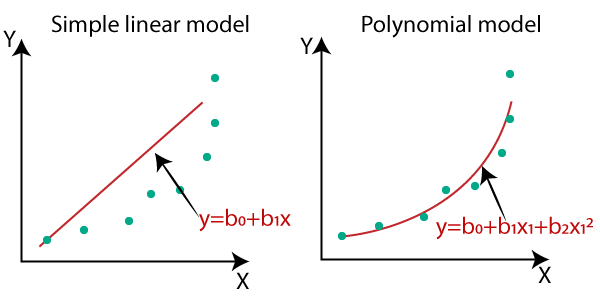
\includegraphics[scale=0.60]{./resources/img/02-regression/polynomial-regression.png}
\end{center}

Note: Why it's still called Linear regression, although we have some non-linearity ?
The answer, the non-linearity comes from the coefficients not the X values.

  \item Non-linear  models
  \begin{itemize}
    \item 
  \end{itemize}

  \item 
\end{itemize}

\begin{mybox}[title={Note: }]
  The Note here
\end{mybox}



\end{document}